\chapter{Discussion and Outlook} % (fold)
\label{cha:conclusions}

\setlength{\epigraphwidth}{8cm}
\renewcommand{\tabcolsep}{0em}

\epigraph{
  \begin{tabular}{p{1.75cm}p{6cm}}
    \footnotesize{\textbf{\textsc{Fry}} :}
      & But I know you in the future.\\
      & I cleaned your poop. \\
    \footnotesize{\textbf{\textsc{Nibbler}} :}
      & Quite possible. We live long and are celebrated poopers. \\
  \end{tabular}
  \vspace{1em}
}{\textit{The Why of Fry}\\ \textsc{Futurama}}

\newpage

\section{Discussion} % (fold)
\label{sec:discussion}

The work done in this project has been evaluated favorably by \emph{the client}, that is, the \ida{T-Labs} staff that asked for this work.
The outcome did fulfill the requirements, so in that sense the project could be qualified as a success.

The developed codebase ended very organized, comparing to other \idx{JavaScript} projects, so it may be easy for others to continue evolving that implementation.
Though hacks and dirty fixes needed to be spilled all over the place because of \ida{IE} quirks and bugs, that did not tarnish the overall architecture.
In conclusion, \idx{MooTools} not only took care of cross-browser issues, but it also helped organizing the codebase.

In the desktop, the resulting interface is much more functional and rich, the user experience has improved a lot and future demonstrations should be a bit more effective.
The fact that no underlying components need to be changed for that is a very nice addition, as it does not complicate the deployment.

The new desktop interface is also very customizable, since the user can move around his devices or the sidebar and leave the interface exactly as he wants.
But it is more important that now the web page can transparently adapt to different screen sizes, because the initial static version was only usable in a big screen.

Another point made in this work is that, with the \ida{HTML}5 and the latest additions to current browsers, it is becoming relatively easy to replace external plugins such as \idx{Java applet}s with plain \idx{JavaScript}.
The developed solution is now more broadly compatible with current devices.

Giving that support for this language is getting increasingly better in all platforms, that the new generation of mobile devices do not run these plugins, and that native SDKs are very heterogeneous between them, the only real cross platform solution will be have to be based on \idx{JavaScript}.
Therefore it is important to verify that web applications can be almost as powerful as any native application.

The mobile version of the app also proves that a mobile web application can be as intuitive as any native application.
The use of elements that are similar to the native elements, not in their appearance but in how they interact, it is very important to create a feeling of familiarity in the user.
The \ida{UI} mechanisms are instantly recognized by the user so he already know how the app works without needing any help.

Once installed, the integration with the \idx{iOS}/\idx{Android} platforms is pretty nice, the user accesses the website exactly as any other native app.
However, the discovery and \emph{installation} of web apps are far less convenient for the user compared to native apps, since there is no web app market integrated into the system.

That and other limitations are only derived of current implementations, there are no technical impediments to create a web application market as the Chrome Web Store\footnote{\url{https://chrome.google.com/webstore}} proves.
In the future, it will be very probable that more platforms will opt for embracing that option.

There is a severe drawback in that mobile version, one that the desktop version do not suffer from.
Although the current generation of mobile browsers is very advanced compared with the previous one, they are still a step behind in efficiency and it is difficult to achieve complete fluidness.

More specifically, the mobile version suffers from a rendering issue with the current \idx{Safari} browser when viewing the content list.
When the user changes to the content list, the browser engine has to render more information than it is designed to handle at once, so it starts painting the elements in blocks (see Figure~\vref{fig:pnai-mobile-sluggish}).

\begin{figure}[htbp]
  \centering
    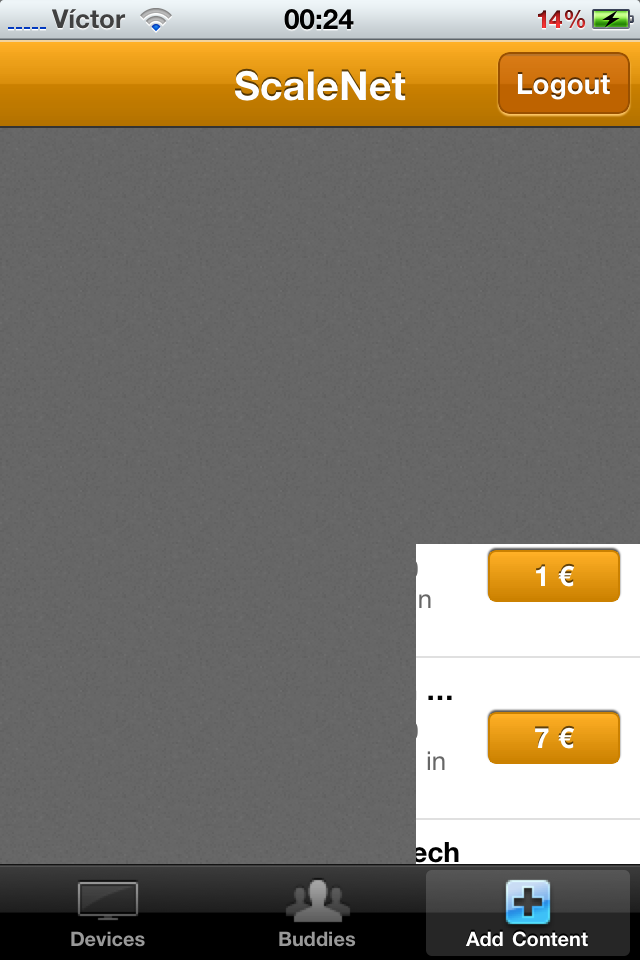
\includegraphics[width=0.24\textwidth]{pnai-mobile-sluggish-1}
    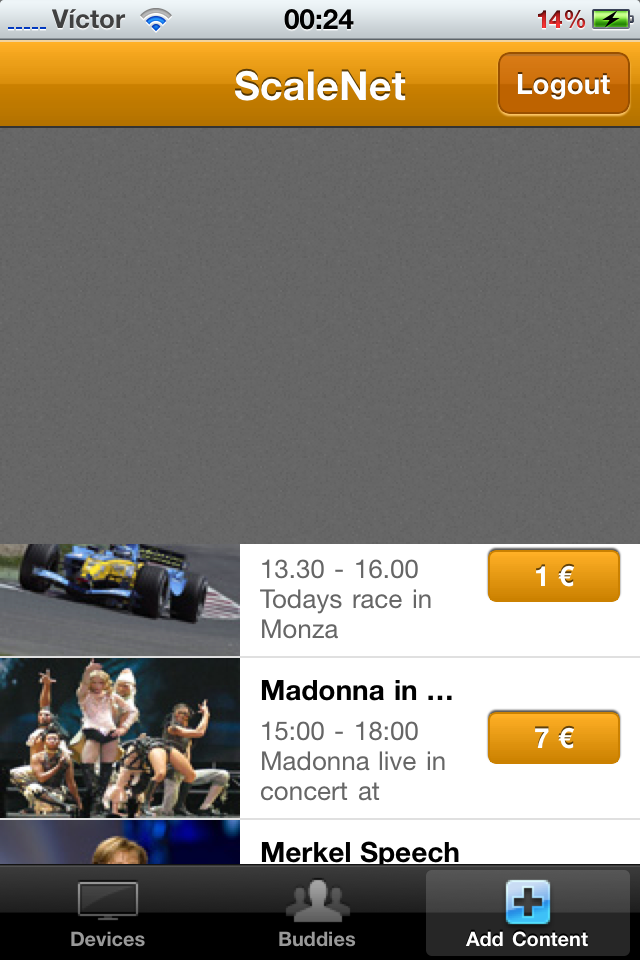
\includegraphics[width=0.24\textwidth]{pnai-mobile-sluggish-2}
    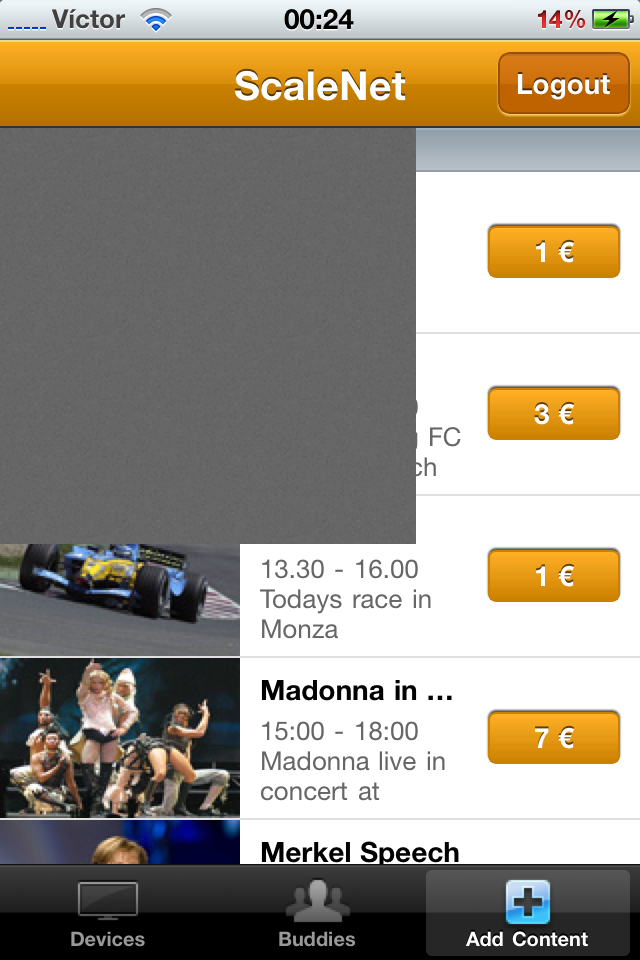
\includegraphics[width=0.24\textwidth]{pnai-mobile-sluggish-3}
    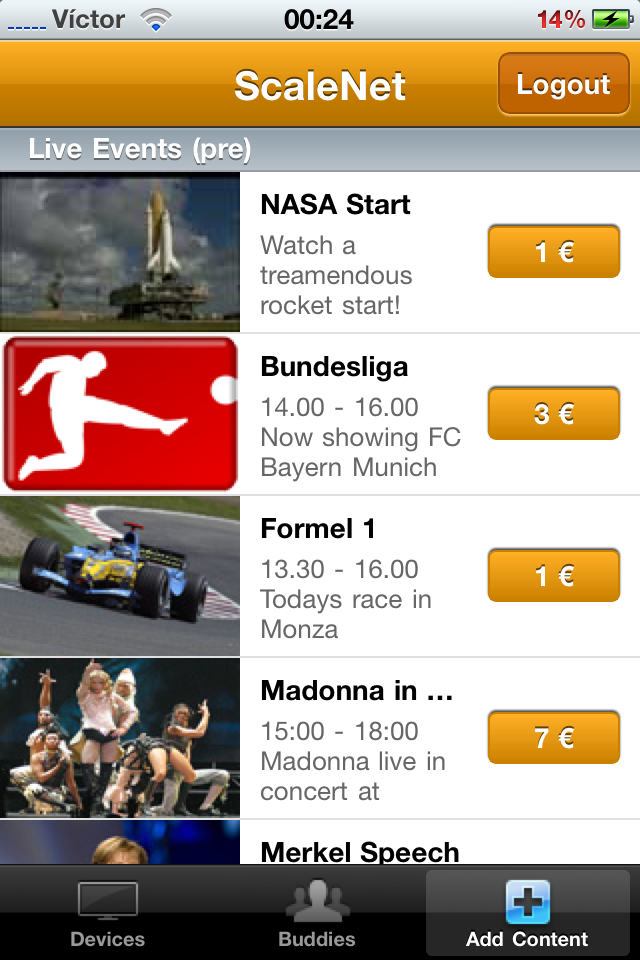
\includegraphics[width=0.24\textwidth]{pnai-mobile-sluggish-4}
  \caption{Rendering issue in the mobile PNAI interface}
  \label{fig:pnai-mobile-sluggish}
\end{figure}

When the view is fully drawn, scrolling still feels sluggish as the new revealed content gets painted.
However, if the content list is scrolled to the end, it can be scrolled without no rendering issue from the beginning, which proves that the browser could handle that web application nicely if we could pre-load the hidden views.

The view is loaded with lots of medium sized images, and certainly the \ida{CSS}3 rules used to paint the buttons does not help, but the root of the problem is the lack of support for fixed positioned element.
That forces us to use the \idx{iScroll} library, adding more overhead as the scrolling has to be done programmatically by \idx{JavaScript} instead of embracing the much snappier native scrolling.

This problem is known by popular mobile applications, and one solution consists of rethinking the interface so that the content is scrolled using the native method, and the tab bar is not fixed but it moves as the browser scrolls.
Google apps like Mobile Gmail or Google Reader used this interface for a while, but it felt kind of weird so they evolved towards more natural approaches.

The real solution to this problem comes with \idx{iOS} 5, as it includes support for fixed elements and native scrolling not only for the whole page but also for inner elements.
Once this update lands, \idx{iScroll} will not be needed anymore and therefore the page can be very fluid keeping the same experience we want.
\nicesectionending
% section discussion (end)

\section{Outlook} % (fold)
\label{sec:outlook}

There is still room for improvements that can be implemented in the application, and the design can be stylized by a professional designer.
In the future, it could be implemented for real users, maybe in a next generation network or in an existing network.
Before that, some shortcomings have to be resolved, like reflecting the real registered devices in the interface for each user.

Like with \idx{IPTVplus}, other \idx{ScaleNet} services could be integrated in the same interface.
Also, it could be interesting to redesign the other pages of the system or even integrate them into the same interface.
For example, it would be useful some controls to manage the devices or the buddies -- adding, editing and removing them -- all in the same place, instead of having to go to external pages.

Looking forward to the future, the mobile version can be reengineered in some ways to make it more responsive.
Since the development was done with an \idx{iPhone}, \idx{Android} only was poorly tested in a simulator.
Therefore, it will be desirable to further test and polish the web application in \idx{Android} devices, Windows 7 phones and even making it bigger for the \idx{iPad} and tablets.

At the same time, other routes can be explored, by converting this web page into a native app.
It would be appealing to evaluate how can this web be ported to native platforms, either by using only native SDKs or by mixing the existing code with native code.
% section outlook (end)
\nicechapterending
% chapter conclusions (end)